\section{Integer-state collapse and rational geometric structure}\label{sec:rational}
This section treats one state. For integers the geometry is determined by one integer and has no topology (\cref{thm:B2T1}); for rationals the realised geometry is determined by the occurrence set (\cref{thm:R3T1a}) but the relations are not (\cref{thm:R3T1,thm:R3T2}).

\subsection{Integer states}
\begin{theorem}[collapse and contractibility of integer states]\label{thm:B2T1}
Let $m$ be an integer with $\sigma=\sigma(m)>1$, let $q_p=\lfloor v_p(m)/2\rfloor=v_p(\sigma)$ and let $k\ge1$ be the number of primes dividing $\sigma$. Then:
\begin{enumerate}[label=(\arabic*),itemsep=1pt]
\item $\Lambda_1=\Z^k$, $\Gr(m)=\{\pm e_p\}$, $\Kmove(m)=\Kaxis(m)$, and the whole record (fibre, lattice, Graver set, cells) is a function of $\sigma$; $\sigma=\max D(m)$ recovers it.
\item $|F|=|D(m)|=\prod_p(q_p+1)-1$; the number of cells is $\prod_p(2q_p+1)-2^k$; $\chi(\Kmove(m))=1$.
\item $\Kmove(m)$ is contractible: its Betti numbers are $(1,0,\dots,0)$.
\item $\Kmove(m)\subseteq\Kmove(m')$ (as cell complexes) iff $D(m)\subseteq D(m')$ iff $q(m)\le q(m')$ coordinatewise.
\end{enumerate}
\end{theorem}
\prov{CW-0395}{B2-T1}{PROVED}{FULL}
\begin{proof}
(1) For $b=1$ every vector satisfies the congruence, so $\Lambda_1=\Z^k$ and $\Gr$ consists of the minimal non-zero vectors of $[-q,q]\cap\Z^k$. A vector with at least two non-zero coordinates dominates, in the conformal order, the unit vector of any one of them, so the minimal vectors are exactly $\pm e_p$ (which lie in the box because every $q_p\ge1$). Hence $\Kmove=\Kaxis$ is the complex of unit cubes of the box $B=\prod[0,q_p]$ none of whose vertices is the origin. The fibre is $B\setminus\{0\}$; everything is read from $q$, equivalently from $\sigma=\prod p^{q_p}=\max D(m)$.

(2) The fibre has $\prod(q_p+1)-1$ points. A cell of the box complex is a pair $(u,S)$, $u\in B$, $S\subseteq\{1..k\}$ with $u+1_S\le q$; in each coordinate there are $q_p+1$ choices if $p\notin S$ and $q_p$ if $p\in S$, in total $\prod(2q_p+1)$ cells. The origin is a vertex of exactly the cells with $u=0$, which are the $2^k$ cells $(0,S)$ (all admissible since $q_p\ge1$). Their contribution to the Euler characteristic is $\sum_S(-1)^{|S|}=0$ and the full box has $\chi=1$, so $\chi(\Kmove)=1$.

(3) Let $B$ also denote the box complex (contractible, being a cell complex structure on a box), $S=[0,1]^k$ the closed star of the origin (all cells containing the origin are faces of $[0,1]^k$) and $K=\Kmove(m)$, so that $B=K\cup S$ and $K\cap S$ is the union of the facets $\{x_i=1\}$ of $S$. All these facets contain the vertex $(1,\dots,1)$, so $K\cap S$ is a cone, hence contractible. Collapsing a contractible subcomplex is a homotopy equivalence (\cite{Hatcher2002}, Prop.~0.17): $B\simeq B/S=K/(K\cap S)\simeq K$. Thus $K$ is contractible.

(4) Cells are determined by their vertices, the vertices are the points of the fibre, and $D(m)=\{p^\alpha\}$ identifies the fibre with $D$. Hence $K(m)\subseteq K(m')$ iff $F\subseteq F'$ iff $D(m)\subseteq D(m')$. If $q\le q'$ then $B\subseteq B'$; conversely $D\subseteq D'$ contains the vertices $p^{q_p}$, giving $q\le q'$. \qedhere
\end{proof}
\begin{remark}[finite-exact check]\label{rem:B2T1check}
The closed forms of (2) and the Betti numbers of (3) were recomputed with the independent engine for the first $700$ integers $m\ge4$ with $\sigma(m)>1$: no exception (\stat{finite-exact}; Appendix~\ref{app:definitions}). The consequence recorded in the programme is that, for integers, \emph{any} geometric law is a law about $\sigma$ and $q$; the topology is trivial. Persistence of occurrence vertices implies persistence of edges and cells for integers; this fails for $b>1$ (\cref{prop:A4T4b}).
\end{remark}
\Cref{fig:integer} shows the exponent box of an integer and its closed-star decomposition .
\begin{figure}[tbp]\centering
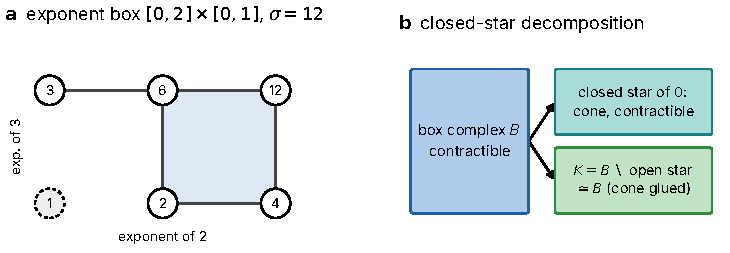
\includegraphics[width=\textwidth]{fig02_integer_collapse}
\caption{\textbf{Integer collapse (exact; proved by \cref{thm:B2T1}).} (a) The move complex of $m=2^4\,3^2\,7$, $\sigma=12$, $q=(2,1)$, drawn in exponent coordinates (a genuine grid embedding): the fibre is the box minus the origin, the shaded square is the unique cell, the dashed vertex $1$ is the removed origin. (b) The closed-star argument for contractibility.}\label{fig:integer}
\end{figure}

\subsection{Rational states: realised geometry is a function of \texorpdfstring{$D$}{D}}
\begin{lemma}[hull lemma]\label{lem:hull}
Let $x$ be a reduced rational, $u,v\in F(x)$ and $g=v-u$. Then $g\in\Gr(x)$ if and only if the coordinate hull $H(u,v)=\{w\in\Z^k:\min(u_i,v_i)\le w_i\le\max(u_i,v_i)\}$ contains no point of $F\cup\{0\}$ other than $u$ and $v$.
\end{lemma}
\begin{proof}
Since $p^u\equiv p^v\equiv1\pmod b$, $g\in\Lambda_b$, and $|g_i|\le q_i$ because $u,v\in B$. Suppose $h\in\Lambda_b$, $h\ne0,g$, $h\sqsubseteq g$. Then $w=u+h$ satisfies $w_i$ between $u_i$ and $u_i+g_i=v_i$, so $w\in H(u,v)\subseteq B$, and $p^w=p^up^h\equiv1\pmod b$, so $w\in F\cup\{0\}$ with $w\ne u,v$. Conversely a point $w\in(F\cup\{0\})\cap H(u,v)$ different from $u,v$ gives $h=w-u\in\Lambda_b$ with $h\sqsubseteq g$, $h\ne0,g$. Hence $g$ is $\sqsubseteq$-minimal in $\Lambda_b\cap[-q,q]$ iff no such $w$ exists. \qedhere
\end{proof}

\begin{theorem}[realised geometry is a function of $D$]\label{thm:R3T1a}
For a reduced rational state $x$, the fibre $F(x)$ is determined by $D(x)$, and the cell complexes $\Kaxis(x)$, $\Kmove(x)$, together with their boundary maps, components and homology, are functions of $D(x)$ alone. Moreover a pair $u,v\in F$ with $g=v-u$ is a $1$-cell of $\Kmove$ iff $H(u,v)\cap(F\cup\{0\})=\{u,v\}$, and every generator of a cell of $\Kmove$ is of this kind.
\end{theorem}
\prov{CW-0409}{R3-T1a}{PROVED}{FULL}
\begin{proof}
$F$ is recovered from $D$ by factorising $d=p^\alpha$. The cells of $\Kaxis$ are the unit cubes with all vertices in $F$. A cell $P(u;g_1,\dots,g_j)$ of $\Kmove$ has all vertices in $F$, in particular $u$ and $u+g_i$ for each $i$; by \cref{lem:hull} the condition $g_i\in\Gr(x)$ is the statement that $H(u,u+g_i)\cap(F\cup\{0\})=\{u,u+g_i\}$, a property of $F$. Linear independence and lexicographic positivity of the generators are properties of the vectors. Hence the set of cells and their boundaries are determined by $F$, and so are all derived invariants. \qedhere
\end{proof}
\begin{remark}[what lies beyond $D$]\label{rem:beyond}
\Cref{thm:R3T1a} concerns the \emph{realised} part of the record. Information beyond $D(x)$ lives in (i) \emph{dormant} Graver vectors (\cref{sec:relations}), (ii) the box and the coordinates of primes that occur in no element of $D$, and (iii) $b$ itself. For integers all of it is a function of $\sigma$ (\cref{thm:B2T1}); for rationals the realised part is not contractible in general (towers, \cref{sec:towertop}) and is generated by the congruence $d\equiv1\pmod b$.
\end{remark}

\subsection{Equal occurrence set, different relations}
\begin{theorem}[occurrence-incompleteness]\label{thm:R3T1}
\emph{(i) Two primes.} Let $r\ge13$ be a prime with $r\equiv5\pmod 8$ and put $x_r=25r^2/(5r-1)$, $y_r=25r^2/8$. Then $x_r,y_r$ are reduced, have the same active primes $\{5,r\}$, the same box $[0,1]^2$ and $D(x_r)=D(y_r)=\{5r\}$, but $\Gr(x_r)=\{\pm(1,1)\}$ and $\Gr(y_r)=\{\pm(1,1),\pm(1,-1)\}$.

\emph{(ii) $k$ primes.} Let $k\ge2$, let $\ell$ be a prime with $k\mid\ell-1$, $c\in(\Z/\ell)^*$ of exact order $k$, and $p_1,\dots,p_k$ distinct primes $\equiv c\pmod\ell$; put $P=\prod p_i$. Then $\ell\mid P-1$, and for $x=P^2/(P-1)$, $y=P^2/\ell$ one has $D(x)=D(y)=\{P\}$, box $[0,1]^k$, $\Gr(x)=\{\pm\mathbf 1\}$ and $\Gr(y)=\{\pm\mathbf 1\}\cup\{e_i-e_j:i\ne j\}$, of sizes $2$ and $k(k-1)+2$.

Both families are infinite: the primes exist, and are infinite in number, by Dirichlet's theorem on primes in arithmetic progressions~\cite{Dirichlet1837}: \emph{if $\gcd(a,m)=1$ then there are infinitely many primes $p\equiv a\pmod m$}. It is applied with $(a,m)=(5,8)$ in (i) and, in (ii), with $(a,m)=(c,\ell)$ (to choose the $p_i$) and with $(1,k)$ (to choose $\ell$).
\end{theorem}
\prov{CW-0410}{R3-T1}{PROVED}{FULL}
\begin{proof}
(i) $\gcd(25r^2,5r-1)=1$ and $\gcd(25r^2,8)=1$, so both fractions are reduced; $v_5=v_r=2$ in both numerators, so $q=(1,1)$ for the primes $(5,r)$. The fibre is contained in $\{(1,0),(0,1),(1,1)\}$. Modulo $b=5r-1$: $5\not\equiv1$ because $0<4<5r-1$; $r\not\equiv1$ because $0<r-1<5r-1$; $5r\equiv1$. Modulo $b=8$: $5\not\equiv1$, $r\equiv5\not\equiv1$, $5r\equiv25\equiv1$. So $F=\{(1,1)\}$ and $D=\{5r\}$ for both. The vector $(1,-1)$ lies in $\Lambda_b$ iff $5\equiv r\pmod b$. For $b=5r-1$ this would need $5r-1\mid r-5$, impossible since $0<|r-5|<5r-1$; for $b=8$ it holds as $r\equiv5$. The vectors $(1,0),(0,1)$ are not in $\Lambda_b$ in either case, so $\Lambda_b\cap[-1,1]^2=\{0,\pm(1,1)\}$ for $x_r$ and $\{0,\pm(1,1),\pm(1,-1)\}$ for $y_r$. The vectors $(1,1)$ and $(1,-1)$ are incomparable in the conformal order, so these sets are the Graver sets.

(ii) $P\equiv c^k\equiv1\pmod\ell$, so $\ell\mid P-1$; both fractions are reduced and the box is $[0,1]^k$. For $x$: for a non-empty $T\subseteq[k]$ put $p_T=\prod_{i\in T}p_i$. If $T\ne[k]$ then $0<p_T-1<P-1$, so $p_T\not\equiv1\pmod{P-1}$; hence $F=\{\mathbf 1\}$. A vector $1_{T_+}-1_{T_-}$ with $T_\pm$ disjoint and non-empty lies in $\Lambda_{P-1}$ iff $p_{T_+}\equiv p_{T_-}\pmod{P-1}$; both numbers lie in $[2,P/2]$ and are different (unique factorisation), so their difference is non-zero of absolute value $<P-1$: impossible. The vectors $1_T$ with $T\ne[k]$ are not in the lattice either. Hence $\Lambda\cap\{-1,0,1\}^k=\{0,\pm\mathbf 1\}$, and $\Gr(x)=\{\pm\mathbf 1\}$ (sub-vectors of $\mathbf 1$ are $1_T$). For $y$: $p_T\equiv c^{|T|}\pmod\ell$, so $F=\{\mathbf 1\}$ and $1_{T_+}-1_{T_-}\in\Lambda_\ell$ iff $k\mid|T_+|-|T_-|$. As $|T_+|+|T_-|\le k$, this means $|T_+|=|T_-|$ or $(T_+,T_-)=([k],\emptyset)$ or the reverse. A vector with $|T_+|=|T_-|\ge1$ dominates $e_i-e_j$ for $i\in T_+$, $j\in T_-$, and $e_i-e_j\in\Lambda_\ell$ is minimal (its proper sub-vectors are $\pm e_i$ or $\pm e_j$, of sum $\pm1\not\equiv0\bmod k$ since $k\ge2$); the vectors $\pm\mathbf 1$ are minimal because $1_T\notin\Lambda_\ell$ for $T\ne[k]$. These are all the minimal elements. \qedhere
\end{proof}
\begin{example}[$r=13$]\label{ex:r13}
$x_{13}=4225/64$ and $y_{13}=4225/8$ both have $D=\{65\}$; $\Gr$ has $2$ resp.\ $4$ elements (\cref{fig:equalD}). For $k=2,3,4$ the sizes $2$ versus $k(k-1)+2=4,8,14$ were recomputed by brute force with the independent engine, for $(\ell;p_i)=(3;5,11)$, $(7;23,37,79)$ and $(5;7,17,37,47)$ (\stat{finite-exact} confirmation of the proved formula).
\end{example}
\begin{figure}[tbp]\centering
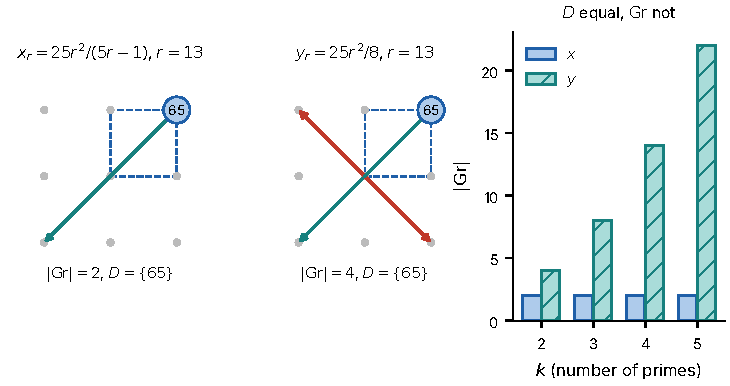
\includegraphics[width=\textwidth]{fig03_equalD_diffGr}
\caption{\textbf{Equal $D$, different Graver sets (exact; proved by \cref{thm:R3T1}).} Left, centre: the exponent plane of $(5,r)$ for $x_r$ and $y_r$, $r=13$; the dashed square is the box, the vertex is $65=5\cdot13$ at $(1,1)$ (the fibre), arrows are the Graver vectors; the red arrows $\pm(1,-1)$ are dormant. Right: sizes of the Graver sets for $x=P^2/(P-1)$ and $y=P^2/\ell$ ($k=2,3,4$ recomputed; $k=5$ is the proved formula).}\label{fig:equalD}
\end{figure}

\subsection{Two primes: the complete classification}
\begin{theorem}[two primes, box $(1,1)$]\label{thm:R3T2}
Let $p<r$ be primes and $x=(pr)^2/b$ with $\gcd(pr,b)=1$. Consider the four statements
\[
A:\ p\equiv1,\qquad B:\ r\equiv1,\qquad C:\ pr\equiv1,\qquad E:\ p\equiv r\qquad(\text{all mod }b).
\]
The lattice $\Lambda_b\cap\{-1,0,1\}^2$ contains $(1,0),(0,1),(1,1),(1,-1)$ exactly when $A,B,C,E$ hold. The set $T\subseteq\{A,B,C,E\}$ of true statements is one of seven:\ $\emptyset$, $\{A\}$, $\{B\}$, $\{C\}$, $\{E\}$, $\{C,E\}$, $\{A,B,C,E\}$; and
\[
\Gr=\emptyset,\ \pm(1,0),\ \pm(0,1),\ \pm(1,1),\ \pm(1,-1),\ \{\pm(1,1),\pm(1,-1)\},\ \{\pm(1,0),\pm(0,1)\}
\]
respectively. Moreover $D=\{p\mid A\}\cup\{r\mid B\}\cup\{pr\mid C\}$. Consequently $D$ determines the type except that $D=\emptyset$ occurs for the types $\emptyset$ and $\{E\}$ and $D=\{pr\}$ for $\{C\}$ and $\{C,E\}$; the bit $e=[E]$ is necessary and sufficient to complete $D$ to the type, i.e.\ $\Gr=\Phi(D,e)$ with $e$ irredundant.
\end{theorem}
\prov{CW-0411}{R3-T2}{PROVED}{FULL}
\begin{proof}
The four vectors are in the lattice iff the stated congruences hold. Lattice closure: $(1,0)+(0,1)=(1,1)$, $(1,0)-(0,1)=(1,-1)$, $(1,1)-(1,0)=(0,1)$, $(1,-1)+(0,1)=(1,0)$. Hence $A\wedge B$ forces $C,E$; $A\wedge C$ forces $B$ and then all; $A\wedge E$ forces $B$ (via $(1,0)-(1,-1)$) and all; $B\wedge C$ forces $A$; $B\wedge E$ forces $A$. The remaining pair $C\wedge E$ forces nothing inside the box (the sum and difference are $(2,0),(0,2)$). Therefore the true sets are exactly the seven listed. If $A$ (resp.\ $B$) holds, $\pm(1,0)$ (resp.\ $\pm(0,1)$) dominates $(1,\pm1)$, which gives the Graver sets of the types $\{A\},\{B\},\{A,B,C,E\}$; for $\{C\}$, $\{E\}$ the lattice contains only $\pm(1,1)$ resp.\ $\pm(1,-1)$; for $\{C,E\}$ the two pairs are conformally incomparable. The fibre points are the vectors of $\{(1,0),(0,1),(1,1)\}$ in the lattice, giving $D$. Necessity of $e$: both values occur for $D=\emptyset$ and $D=\{pr\}$ (\cref{ex:twoprime}); sufficiency: the table. \qedhere
\end{proof}
\begin{example}[both values of $e$ occur]\label{ex:twoprime}
$(p,r,b)=(5,13,8)$: $E$ holds ($13\equiv5$), $C$ holds, $D=\{65\}$, type $\{C,E\}$. $(p,r,b)=(5,13,64)$: only $C$, $D=\{65\}$, type $\{C\}$. For $D=\emptyset$ (neither $A,B,C$): $(p,r,b)=(3,7,4)$ gives $3\equiv7\pmod 4$, type $\{E\}$ ($\Gr=\pm(1,-1)$, no occurrence), whereas $(3,7,5)$ gives type $\emptyset$.
\end{example}
\begin{remark}[finite-exact confirmation]\label{rem:R3T2check}
For $p\in\{2,3,5,7,11,13\}$, $r\le23$ prime, $2\le b<120$, $\gcd(pr,b)=1$, the engine computed $\Gr$ by brute force for $2{,}620$ states: the type table holds for every state, and only the seven types occur, with counts $2339,27,56,108,24,32,34$ for $\emptyset,A,B,C,E,CE,ABCE$ (\cref{fig:twoprime}; \stat{finite-exact} confirmation, Appendix~\ref{app:relations}).
\end{remark}
\begin{figure}[tbp]\centering
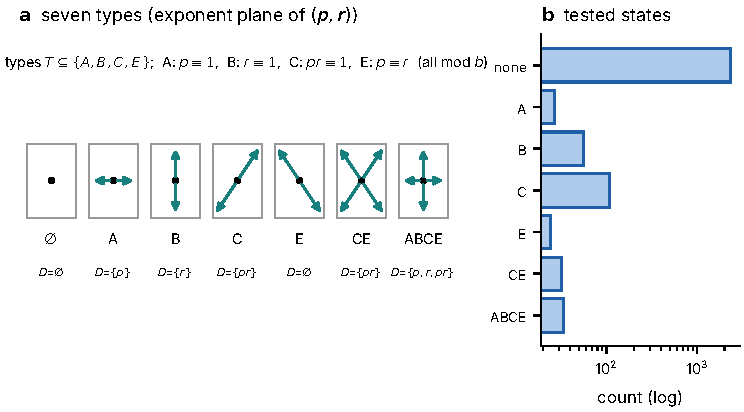
\includegraphics[width=\textwidth]{fig04_two_prime_types}
\caption{\textbf{The seven two-prime types (exact; proved by \cref{thm:R3T2}).} (a) The Graver vectors (arrows in the exponent plane of $(p,r)$) and the occurrence set of each type. (b) Number of tested states of each type among the $2{,}620$ states of \cref{rem:R3T2check} (finite-exact; log scale).}\label{fig:twoprime}
\end{figure}
\begin{problem}[R3-T2$'$: beyond two primes]\label{prob:R3T2p}
Classify the minimal descriptor $\Phi(D,J)$ beyond $D$ (the set $J$ of dormant relations) for boxes $q\ne\mathbf1^k$ and for three or more primes in full generality. Family (ii) of \cref{thm:R3T1} shows that for $q=\mathbf 1^k$ the dormant set can be the whole root system $A_{k-1}$, so the answer is a statement about lattice types, not about the number of coordinates.
\end{problem}
\prov{CW-0412}{R3-T2'}{OPEN}{OPEN}
